\documentclass[a4paper,10pt]{article}
\author{Cristiano Morais Monteiro}
\title{Cloud Computing}
\usepackage{fullpage}
\usepackage{listings}
\usepackage{graphicx}
\usepackage{hyperref}
\usepackage{color}
\usepackage{blindtext}
\usepackage[inline]{enumitem}
\usepackage{xcolor}
\usepackage{tasks}
\usepackage{ragged2e}
\begin{document}
\maketitle
\newpage
\justify
\tableofcontents
\newpage
\ part{Lernheft 1}
\section{Lektion 1}
Im cloud computing werden Anwendungen (Programme) auf entfernten Rechnern ausgeführt. Der Begriff Datenwolke wird verwendet weil Daten auf entferntern Rechnern gespeichert werden. \newline
Cloud Computing ermöglicht:
\begin{itemize}
	\item Bereitstellung von Anwendungen (in der Cloud ausgeführt), Diensten und Speicherkapazitäten
	\item Daten remote zu speichern
	\item Eigene Anschaffung von Hardware und Software ist nicht mehr notwendig (darum günstig)
\end{itemize}
Ein Beispiel wäre: \newline
Unternehmen X hat App Y entwickelt. Unternehmen X ist Kunde von Amazon und nutzt deren Amazon AWS cloud Dienste (Dienste, Speicherkapazität und Computing). Unternehmen X hat tausende von Kunden. Falls die Kundenanzahl von X sinkt, sinkt der Bedarf von X an Cloud Ressourcen die von Amazon bereitgestellt werden. Dadurch muss Unternehmen X da es weniger Cloud Dienste nutzt auch weniger an Amazon bezahlen (Skalierbargkeit \textit{``On-Demand''} der Cloud).
Cloud Computing ist sehr dynamisch, durch die Verwendung von Cloud Diensten muss X nicht mehr:
\begin{itemize}
	\item Hardware skallieren rauf/runter verbunden mit der Anzahl der Kunden
	\item Kann den Dienst sehr einfach und sofort der Kundenanzahl anpassen
\end{itemize}
\vspace{3mm}
Es gibt hauptsächlich drei Arten von Cloud Computing:
\begin{itemize}
	\item SAAS - Fertige Anwendungen (Email, office, \ldots).
	\item PAAS - Liefert Datenbanken und Webdienste auf die eigene Anwendungen entwickelt werden können.
	\item IAAS - Liefert Rechenkapazität (computing), Speicher und Netzwerk Anbndungen.
		\begin{itemize}
			\item Kann bereitgestellt werden/umgesetzt on/off-Premise, können Public (Dropbox, Gmail=SAAS), private, Community oder Hybrid Clouds sein aka Bereitstellungsformen.
		\end{itemize}
\end{itemize}
Ziel des Cloud computing ist es Rechen- und Speicherkapazitäten so einfach bereit zu stellen, wie Strom aus der Steckdose.
\vspace{3mm}
Da dir Übertragung von Strom teuerer ist als die Übertragung von Daten und die Einrichtung/Wartung eines eigenen Rechenzentrum sehr sehr teuer ist kann man behaupten das große zentrale Rechenzentren ``effizienter'' als mehrere kleine sind.
\vspace{3mm}
Eine Private Cloud ist stren genommen gar keine Form von Cloud Computing, da das Element Fernstreckanbindung fehlt.
Bezüglich der Flexibilität is die \textit{Public Cloud} die am geringste flexible Bereitstellungsform und \textit{Private Cloud die am Flexibilsten}.
\vspace{3mm}
Wenn mann eigene IT-Dienste mit Ressourcen der Eigenen Privaten Cloud (lokale Cloud Technologie) als auch mit Ressourcen einer Public Cloud bereit stellt, nennt mann dies eine \textit{Hybrid Cloud}. On-Premise bedeutet das Software/Dienste im eigenen Haus bereitgestellt werden. Off-Premise bedeutet das diese in einem entfernten gebäude/Rechenzentrum bereitgestellt werden. \vspace{3mm}
Eine Community Cloud ist nicht das selbe wie eine Hybrid Cloud. Eine Community beschreibt lediglich die Bereitstellung von Cloud diensten für mehrere Kunden/organizationen mit ähnlichen Sicherheitsanforderungen wie z.B öffentliche Verwaltungen.

\subsection{Aufgaben}
1.1 - Welche Klassen von Cloud Computing gibt es? \newline
R: \textit{SAAS, IAAS, PAAS.} \break
1.2 - ``On Premise'' bereitgestellte Anwendungen und Dienste werden im eigenen Rechenzentrum betrieben - richtig oder falsch? \newline
R: \textit{JA} \break
Welche Bereitstellungsformen von Cloud Computing sind flexibler als Public Cloud? \break
R: \textit{Community, Hybrid und Private}

\section{Lektion 2}
Hardware Virtualisierung (VMware) besteht aus zweit typen:
\begin{itemize}
	\item Type 1 auch \textit{``Bare Metal''} gennant
		\begin{itemize}
			\item performanter, Hypervisor läuft direkt auf Hardware. Hypervisor verfügt/muss über/haben notwendige Treiber für die Hardware
		\end{itemize}
	\item Type 2 auch ``hosted'' gennant.
		\begin{itemize}
			\item Hypervisor wird auf einem bestehenden Betriebssystem installiert. Treiber werden vom OS bereitgestellt. Weniger performant als Type 1.
		\end{itemize}
\end{itemize}
Software Virtualisierung (App-V). Moderne Virtualisierung verfügt über Funktionen wie \texttt{Live Migration/V-Motion} die es ermöglichen VMs ohne Downtime ``umzuziehen''. Im fall von Storage-VMotion wechselt die Ganze VM den Speicherort.
\vspace{3mm}
Weil es ja mehrere Arten von Cloud Computing gibt entstehen aus seite des Anbiters mehrere verschiedene Angebote/Packete. Um diese differenzieren zu können werden Schichtmodelle verwendet:
\begin{itemize}
	\item OSI - rein theoretisches Modell
	\item TCP/IP - Implementierungsmodell
\end{itemize}
im TCP/IP modell wird von unter nach oben gezählt:
\begin{enumerate}
	\item Netzwerk - Physische Verbindung; Bit-Übertragung über das jeweilige Medium (Kabel, Faser, Funk); Fehlerkorrektur durch checksummen.
	\item Routing
	\item IP; TCP; UDP
	\item Spezifische Protokolle der Anwendungen HTTP; SMTP; VOIP.
\end{enumerate}
Für Cloud Computing ist layer 3 und 4 am wichtigsten da hier Verschlüsselung angewendet werden kann. \texttt{IPSEC} kann in L3 eingesetzt werden, da dies aber für tausende von Kunden zu einem zu hohen Aufwand führt, wird die Verschlüsselung auf L4 betrieben durch SSL/TLS oder SSH, durch den Browser insbesondere wenn SAAS verwendet wird. Herausforderung für das Cloud Computing ist die Datensicherheit, genauer der Transport der Daten durch das Internet, in der Cloud gespeicherte Daten sollen nicht für andere außer den Kunden verfügbar sein (auch nicht Admin).
\vspace{3mm}
Die verschiedenen VPN Typen sind:
\begin{itemize}
	\item End-to-End: PC zu PC, oft in SAAS verwendet; SSL (Browser)
	\item End-to-Site: PC zu Netz ; IAAS
	\item Site-to-Site: Netz zu Netz
\end{itemize}
Site-to-Site Beispiel: \newline
Amazon Elastic Compute Cloud (EC2) in der man als Kunde eine Virtual Private Cloud (VPC) erstellen kann, die dann über eine VPN Gateway mit dem eigenen Netz verbunden wird.
\vspace{3mm}
Speichervirtualisierung wird haptsächlich in SANs eingesetzt. Eine \texttt{SAN} beschreibt mehrere verbundene Speichersysteme die ein Speichernetz bilden. Die einzelnen Speichersysteme haben mehrere Festplatten. Durch die verwendung von SAN ist die Speicherverwaltung viel einfacher da nicht mehr einzelne Festplatten in Servern erweitert oder gewartet werden müssen.
\vspace{3mm}
Ein bestehendes Problem auch mit SANs ist die Speicherauslastung. Deswegen wurden technologien wie \textit{Thin Provisioning} entwickelt. Thin Provisioning im Gegensatz zur üblichen \textit{Vollständigen Zuordnung (Thick Provisioning)} wird bei der schlanken Speicherzuweisung nur der Speicher reserviert, welcher auch tatsächlich benötigt wird. Dadurch kann ``schneinbar'' mehr Speicher bereitgestellt werden, als tatsächlich vorhanden ist. Trotzdem muss die Storae-Pool überwacht und gewartet werden. Falls diese keinen freien Speicher mehr hat sind die Volumes nicht mehr schreibbar. Aufgrund der starken Konzentration von Speicher sind bei der Verwendung von Speichernetzten mehrere (manchmal sogar alle) Server von der Verfügbarkeit der Speicherdienst abhängig. Was eine Nachteil diese Technologie im Gegensatz zu üblichen Festplatten in den einzelnen Servern. \newline
Um dieses Problem beizukommen wurden verschiedene Spiegelmechanism entwickelt: \begin{itemize}
	\item Synchrone Datenspiegelung  - Es wird gleichzeitig auf die gespiegelten volumes geschrieben. Ein Schreibvorgang ist erst dann beendet wenn es auf beiden beendet wurde.
		\begin{itemize}
			\item Aktiv-Aktiv: Automatisches FailOver bei Ausfällen.
			\item Aktiv-passiv: Manuelle Intervention ist erforderlich für den Failover bzw. Bereitstellung und Pfade anpasen.
		\end{itemize}
	\item Asynchrone Datenspiegelung: Die schreibvorgange werden nachgelagert jeweils auf dem Volume geschrieben; kein automatisches Failover. Wird oft in weiten Strecken verwendet.
\end{itemize}

Innerhalb der Welt des Cloud Computings sind Speichervirtualisierungstechnologien in Private und hybrid Clouds sowie IAAS - Angebote zu Hause.
\vspace{3mm}
Bei der Hardware- / Servervirtuakisierung ist die virtuelle Hardware immer die selbe (aber mehrere Instanzen davon) für jede VM. Treiber suchen, installieren fällt weg. Dafür sollten aber die Hypervisor Kompatibilitätslisten vor einer Einführung untersucht werden. \newline
Alle server Hardware Hersteller wollten, das ihre Hardware kompatible mit Servervirtualisierung ist. Dadurch hat als Nebeneffekt eine Server Hardware Standardisierung stattgefunden.
\vspace{3mm}
Der Vorgang bei einer \texttt{Live Migration/VMotion} ist folgender:
\begin{enumerate}
	\item Ein vollständiger Snapshot des Arbeitspeichers der Quell VM wird durchgeführt und eine Leere VM im Zielsystem angelegt.
	\item Der Snapshot wird dann auf das Ziel VM gespielt.
	\item Ein inkrementeller Snaphsot wird an der Quell VM durchgeführt und Übertragen zum Zielsystem
	\item Der inkrementelle Snapshot wird auf die Ziel VM gespielt um die letzten Änderungen (Änderungen seit  begin des Prozesses) auf der verschobenen VM zu haben.
\end{enumerate}
Eine Festplattendatei- oder Datenverschiebung findet hier nicht statt da für eine Live-Migration/VMotion eine shared Storage verwendet wird. IP/MAC bleibt gleich! (in vFestplatte). \newline
Bei \texttt{Storage-VMotion} hingegen wird der ganze Speicherort der VM bzw. die Festplattendatei geändert. Die notwendigen Dateine werden verschoben. Aber auch hier gibt es kein Downtime.
\begin{enumerate}
	\item Snapshot mit den neuesten Änderungen wird erstellt und dann an Zielspeicherort übertragen
	\item Festplattendatei wird verschoben
	\item neueste Snapshot und Festplattendatei werden zusammengeführt.
\end{enumerate}
Durch die Verwendung von VMs wird der Backup- und Wiederherstellungsprozess deutlich vereinfacht( nur wenige Dateien müssen gesichert werden, Snapshot gibt es auch noch).
\vspace{3mm}
\texttt{Desktopvirtualisierung ( nicht gleich TS; VDI) -- Nutzerdaten sind in der Cloud} \newline
Der Mehrwert der Desktopvortialisierung besteht darin, dass die Nutzer sich nicht beim TerminalServer ein Betriebssystem teilen müssen, sondern jeder Nutzer sein eigenes Betriebssystem benutzt. Dies führt dazu, dass jeder Benutzer die Systemeinstellungen seiner virtuellen Maschine nach Herzenslust verändern kann und auch seine eigenen Anwendungen installieren kann, ohne die anderen Nutzer, die sich mit ihren Sitzungen auf derselben Hardware aufhalten, zu beeinflussen.

\texttt{Applikationsvirtualisierung (Sandboxing, App-V)} -- Nutzerdaten sind lokal \newline
Der Mehrwert hier besteht darin, Anwendungen in sogenannten Sandboxes auszuführen und somit voneinander abzuschotten. Dadurch kann mann Anwendungen auf dem selben System bereitstellen die normalerweise nicht auf dem selben System installiert werden dürfen. Dies stellt einen erheblichen Mehrwert in Terminalserver-Farmen dar, da dadurch die Anzahl der benötigten Terminalserver verringert wird. Ein weiterer Mehrwert besteht darin das neue Anwendungen hinzugefügt werden können, ohne hierfür Installationsroutinen aufrufen zu müssen. App-v erlaubt es sogar Anwendungen über das Internet zu streamen. Die Nutzerdaten bleiben lokal.
App-V(containerization oder eigene VM) != Remote-Desktop app \newline

\vspace{3mm}
Ein Nutzerprofil ist, einfach ausgedrückt, ein Satz aus Einstellungen, die der Nutzer während der Benutzung seiner Anwendungen vorgenommen hat. Microsoft hat in seinen Windows-Betriebssystemen eine Funktion mit dem Namen ``servergespeicherte Profile'' (engl. ``Roaming Profile'') integriert, die es den Nutzern erlaubt, ihr Profil von einem Computer zum nächsten mitzunehmen. Der Vorteil ist das der Benutzer jedes er sich auf einem anderen Terminalserver befindet seine Einstellungen durchführen müss und fürt zu weniger Datenredundanz auf den Servern. Ein Beispiel wie dies funktioniert ist:
\begin{enumerate}
	\item Der Nutzer vebindet sich zum Server
	\item Der TS fragt Domain Controller nach dem Speicherort des Profils des Nutzers.
	\item Der DC gibt einen UNC PFAD zurück (FileServer)
	\item Der Terminalserver lädt das Profil von dem angegebenen Server.
	\item Bei der Abmeldung des Nutzers vom TS wird das verändert Nutzerprofil zurück auf den Dateiserver gespeichert.
\end{enumerate}
Appsense = Nutzerdaten werden in Datenbank gespeichert und der schreibende Zugriff auf das profil durch mehrere gleichzeitig geöffneten TS sitzungen ist möglich.

\subsection{Aufgaben}
3.1 - Aus vier: Netzwerk(physikalische Verbindung), Internet(routing), Transport(IP,UDP,TCP) und Anwendung \break
3.2 - ab Transport bzw. Layer 3. \break
3.3 - End-to-Site. \break
3.4 - Falsch, mit Thin-Provisioning kann die Auslastung von Speicher erhöht werden. \break
3.5 - Aktiv-Aktiv; Aktiv-Passiv; Failover. \break
3.6 - Hardware-/Servervirtualisierung. Easy backup and Recovery, lower Costs, lower workload. \break
3.7 - 5 Betriebssysteme werden für 5 Sitzungen ind Desktopvirtualisierung benötigt (VDI) \break
3.8 - Falsch \break
3.9 - Richtig, nicht auf der selben Maschine, keine Datenredundanz.
\section{Lektion 3}
Die Innovationskraft des Internets kommt einzig und allein aus einer Einfachheit und vor allem aus einer Offenheit. Das Internet selbst muss nicht geändert werden, um eine neue Anwendung zu unterstützen. Der Einzige der umsetzen und von der Idee überzeugt sein muss, ist der Innovator selbst. Aufgrund der Einfachheit und Offenheit des Internets fehlt z.B eine Möglichkeit, die Qualität einer VPN-Verbindung zwischen dem eigenen Rechenzentrum und der ``Virtual Private Cloud'' (bzw. dem Cloud Provider) zu garantieren.
\vspace{3mm}

Die größten Bedenken zum Thema Cloud Computing bestehen bezüglich der Datensicherheit -- Die meisten Unternehmen möchten ihre Daten lieber im eigenen Rechenzentrum speichern und nicht über das Internet transportieren und in der ``Cloud'' speichern. Die verschiedenen Bereitstellungsformen des Cloud Computings unterscheiden sich erheblich in ihrer Datensicherheit. Das ist klar bei z.B einer Private Cloud wo keine Daten über ein externes Netzwerk transportiert werden müssen. Zu Unternehmenskritischen Daten zählen zum einen die Daten, die zur Authentifizierung, wie Forschungsergebnisse oder Quellcode von Software. Es muss sichergestellt werden das Daten nicht mitgelesen werden können. Was bedeuted die Daten müssen über eine Verschlüsselte Verbindung übertragen werden. Lösungen hierfür sind Site-To-Site VPNs und SSL-Verbindungen. Es darf unter anderem nicht möglich sein, dass ein Kunde, der ein SAAS-Angebote zum Thema CRM nutzt, Zugriff auf die Kundendaten eines anderen Kunden bekommt. D.h., die angebotene Software muss eine sichere Mandantenfähigkeit mitbringen. Administratores des Rechenzentrums dürfen auch keinen Zugriff auf Kundenspezifische Daten haben. Eine Technische lösung besteht darin, dass der Kunde des Cloud Service Providers sine Daten selbst verschlüsselt.
\vspace{3mm}
Zuätzlich zu Datensicherheit, muss der Provider darlegen, wie er Datensicherungen und Datenwiederherstellungen durchführt. Oft vergissen wird, dass der Provider auch eine Möglichkeit anbieten sollte die Kundendaten im Rechenzentrum ``exportierbar'' zu machen, falls der Kunde einen On-Premise Betrieb wieder aufnehmen möchte. Es ist zumindest in Deutschland nicht erlaubt (ohne Zustimmung des Kunden), Finanzdaten von Kunden außerhalb von Deutschland zu speichern.
\vspace{3mm}
Der Cloud Provider darf auch den Physikalischen Sicherheits Aspekt nicht verschlafen und Zugangskontrollen mit Protokollisten im Rechenzentrum führen. Eine ähnliche Zugangskontrolle und Protokollierung muss auch auf Digitale Ebene stattfinden, sodass immer bewusst ist welche Admin auf welche System gerade zugreift oder zugegriffen hat.
\vspace{3mm}
Eines der Meistgenutzten Argumente für das Cloud Computing ist der Umweltschutz. Aufgrund der hohen Effizienz von neuen großen Rechenzentren kann mehr Leistung mit weniger Energie gezahlt werden. Und weniger Energieaufnahme bedeutet weniger CO2. Der Cloud Service Provider Goolag geht hier mit gutem Beispiel voran und betreibt seine Rechenzentren ausschließlich mit erneubaren Energiequellen (Wasser, Wind und Solar). Cloud Provider müssen dafür sorgen, dass die vorhandenen Rechenzentren maximal ausgelastet werden, sodass nicht mehr Rechenzentren gebaut werden müssen, als unbedingt notwendig.

\subsection{Aufgaben}
4.1 - Jerome H. Saltzer, David P. Reed und David D. Clark.
\vspace{3mm}

4.2 - Richtig
\vspace{3mm}

4.3 - Da es zu einem ungerechtem Konkurrenzkampf führen kann und die Innovationskraft des Internets einschränken könnte.
\vspace{3mm}

4.4 - richtig
\vspace{3mm}
4.5 - falsh, wenn es sich um Finanzdaten handelt. Dafür benötigt man die Erlaubnis des Kunden
\vspace{3mm}

4.6 - Falsch, auch die Menge und Energiequelle bzw. ob Erneubare Energie als Quelle verwendet wird.

\part{Lernheft 2}

\section{Lektion 1}
Virtuelle Maschinen werden unter anderem für die Hardwarevertualisierung eingesetzt. Dabei werden Betriebssysteminstanzen von der Hardware getrennt. Dazu baut eine spezielle Virtualisierungsschicht quasi einen Computer nach. Der Computer, auf dem eine VM läuft, wird auch \texttt{Host} genannt. Mit einem entsprechend leistungsfähigen System können Sie dabei auch mehrere Computer simulieren. Jeder dieser simulierten Computer arbeitet dabei komplett isoliert von den anderen simulierten Computern.
\vspace{3mm}
Virtuelle maschinen sind wichtig für Cloud Computing, aus mehreren Gründen:
\begin{enumerate}
	\item Sie ermöglichen eine sehr ökonomische Auslastung vorhandener Hardware. Durch mehrere virtuelle Maschinen, die gleichzeitig auf einem sehr Leistungsfähigen server arbeiten, kann die oft sehr teure Hardware sehr viel besser genutzt werden. Der Stromverbrauch und der Aufwand für die Kühlung werden auch sehr stark verringert.
	\item Sie ermöglichen einen sehr einfachen Umzug von kompletten Servern. Virtuelle Maschinen bestehen in der Regel nur aus einigen Dateien. Diese Dateien lassen sich ganz normal kopieren--auch zwischen verschidenen physischen Computern. Live Migration gibt es ja auch noch.
	\item Sie ermöglichen eine sehr einfache Datensicherung und -wiederherstellung.
	\item Sie können sich ein eigenes virtuelles Netzwerk aufbauen zum testen. Mit mehrere VMs auf die sie über das Netzwerk zugreifen können.
\end{enumerate}
\vspace{3mm}
Als Betriebssystem erwartet der VMware Worksation Player, mindestens Windows 7. Unterstützt werden nur 64-Bit Versionen. Als Gastsystem können sie neben aktuellen WIndows-Versionen auch ältere Windows-Versionen oder Linux Distros installieren.
\section{Lektion 3}
Auch für die Installation eines Betriebssystems oder einer Anwendung in einer VM gelten in der Regel die Lizenzierungsbedingungen des Herstellers. So dürfen Sie bei einer Standardlizenz zum Beispiel die meisten Windows-Versionen nur auf einem Rechner installieren und nutzen. Dabei spielt es keine Rolle, ob die Intallation auf einem ``echten'' Rechner erfolgt oder in einer VM. Für die Installation von MS Server 2016 ist keine besondere Lizenz erforderlich. Die Testversion von Windows Server 2016 ist grundsätzlich nahezu drei Jahre lang lauffähig. Allerdings müssen Sie die Testphase merfach verlängern.
\vspace{3mm}
Die virtuelle Machine übernimmt auch die Steuerung der Tastatur, wenn Sie mit der Maus in das Fenster klicken. Um die Steuerung wieder an den Host zu übergeben, klicken Sie mit der Maus an einer beliebigen Stelle außerhalb des Fensters der Virtuellen Maschine oder STRG+ALT drücken. Die Tastenkombination STRG+ALT+Entf können sie in einer Vm nicht verwenden.
\vspace{3mm}
Damit die Arbeit der virtuellen Maschine flüssiger und konfortabler abläuft, sollten sie noch die VMWARE TOOLS installieren. Es handelt sich um spezielle Erweiterungen, die zum Beispiel Treiber für eine bessere virtuelle Grafikkarte und verschiedene Sonderfunktionen zu Verfügung stellen.


Dateien zwischen Host und Gast können Sie problemlos durch Drag and Drop oder auch über die Windows-Zwischenablage austauschen. Wenn sie viele Dateien austaschen müssen zwischen Host und Gast können sie auch einen Ordner auf dem Host für die VM freigeben. (Netzlaufwerk). Sie können an den Symbolen rechts in der Symbolleiste des VMware Workstation Plyers erkennen, ob Aktivitäten stattfinden. Bei zugriffen auf die Festplatte erscheint zum Beispiel ein kleines Festplatten Symbol mit einem grünen Ball. Bei Zugriff auf das Netzwerk wird auch dieser grüne Ball angezeigt auf dem Netzwerksymbol.


Mit dem PowerShell befehl \textit{slmgr /rearm} wird die MS WIndows Server 2016 Testphase verlängert.



















































\part{Lernheft 3}
Bei der Nutzung von Cloud-computing-Produkten sind stets mindestens zwei Betriebssysteme im Einsatz -- eines auf dem die Cloud-Dienste zugreifenden Endgerät und eines auf dem Cloud-Dienste bereutstellenden Server.
\section{Cloud-OS für Rechenzentren}
Es gibt zwei arten von Cloud-OS:
\begin{enumerate}
	\item Das Cloud OS für Rechenzentren
		\begin{itemize}
			\item Wurde zuerst von VMware erfunden.
			\item Mit der Einführung von ESXi, einem Bare-metal-Hypervisor, fing VMware an, dieses Produkt als Cloud OS zu bezeichnen
			\item Die idee hinter dieser Bezeichnung geht darauf zurück, dass man mehrere ESXi Server zu einer Coud zusammenfassen kann (ESXi-Verbund; was denn mit Vcenter verwaltet wird). Da bei einem Verbund dieser Art es zwanghast Shared storage gibt kommt hier due Funktion Live-Migration ins Spiel.
			\item Zusammen mit einer Funktion zur automatischen Lastverteilung (in den VMware-Produkten wird diese Funktion Distributed Resource Scheduling, kurz DRS genannt), die automatisch virtuelle Maschinen, je nach Last auf der im ESX-Verbund (cloud) vorhandenen Serverhardware verteilt.
			\item Dies führt zu einem Zustand, bei dem es keine eindeutige zuordung zwischen Serverdienst(Instanz+Anwender Dienst/Produkt) und Serverhardware mehr gibt. Die Zusammengeschaltete Serverhardware wird zu einer Cloud, die zum Betrieb der Diesnte genutzt werden kann.
				\begin{center}
					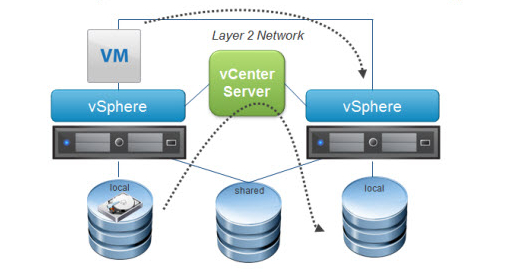
\includegraphics[width=5in,height=3in]{esxiverb.jpg}
				\end{center}

			\item Die VMs können auf einem beliebigem ESX Server laufen der teil des ESX verbunds ist. Dafür benötigt mann nur shared storage zwischen den ESXI. Durch DRS und Live Migration wird VM anhand der Last herumgeschoben.

			\item Cloud-OS Für Rechenzentren unterscheidet sich sich von herkömmlichen Server-betriebssystemen dahingehend, dass in dem Betriebssystem selbst keine ``normalen'' Serverdienste (z.B DNS, DHCP, Active Directory) enthalten sind. Vielmehr sind diese stark spezialisierten Betriebssysteme darauf ausgelegt, einen möglichst geringen Footprint aif der Serverhardware zu hinterlassen und sich auf die Resourcen-schonende Bereitsstellung von VMs zu konzentrieren.
			\item ``Footprint'' = Je weniger Speicherplatz, RAM Vernrauch und weniger CPU-Last die Software/System selbst erzeugt, umso kleiner ist der Footprint der Software. Bei einem Hypervisor bedeutet dies, das mehr VM Instanzen laufen können aus der Hardware bzw. besser Hardware Auslastung. Immer zu betrachten aber, sind die Hardwarekompatibilitätslisten des Hypervisors.
		\end{itemize}

	\item Cloud-OS für Endgeräte
		\begin{itemize}
			\item Einsatzzweck der Cloud-OS für Endgeräte ist es, dem Nutzer ein möglichst einfaches und wartungsarmes Betriebssystem zu Verfügung zu stellen, mit dem er seine in der Cloud betriebene Software (SaaS-Angebote) ausführen kann.
			\item Chromium OS (Google) ist für die Nutzung auf Netbooks konzipiert und wurde um den Chrome Webbrowser herum entwickelt. Chromium-OS, ist open-source und ist für Entwicklet gedacht. Neben Chromium-OS produziert google aChrome-OS, das als vorinstalliertes Betriebssystem auf den Netbooks verschiedener Hardwarehersteller verkauft wird.
			\item Android und iOS (sowie alle Mobilen-Betriebssysteme) unterscheiden sich von Chromium-OS durch die Möglichkeit, mehrere Anwendungen aus dem entsprechenden App-Store herunterzuladen und auf dem Endgerät lokal auszuführen. Auch wenn die meisten dieser Anwendungen für ihre Funktionalität eine Internetverbindung voraussetzen, um einen entsprechenden Cloud-Dienst zu erreichen, werden diese Betriebssysteme bisher nicht als Cloud-OS bezeichnet.
		\end{itemize}


	\item Beide Arten haveb gemeinsam, dass die Entwicklet der Betriebssysteme versuchen, den Footprint der Software zu minimieren.
\end{enumerate}
\vspace{3mm}
Cloudready ist Chromium-OS basierend, und wird von Neverware betrieben. Es steht auch als .OVA Virtual Appliance verfügbar.Die Namenserweiterung OVA steht für Open Virtualization Archive. Dabei handelt es sich um ein Format für den Austausch von Software, die in virtuellen Maschinen läuft. \textit{Eine Virtual Appliance ist eine lauffähige vorinstallierte und vorkonfigurierte virtuelle Maschine. Diese können Sie nach dem Import direkt starten.} Bei Fehlkonfiguration eine Virtual Appliance kann dieser einfach erneut importiert werden.
\vspace{3mm}
Wie bereits erwähnt, bei einem Cloud-Betriebssystem für Endgeräte werden Anwendungen nicht lokal installiert und ausgeführt, sondern, dass vor allem Dienste im Internet damit genutzt werden können. Dafür ist eine Verbindung mit dem Internet obligatorisch. Chromium-OS wurde für die Nutzung mit den von Google angebotenen SaaS-Produkten entwickelt. Um alle Funktionen nutzen zu können müssen Sie sich mit ihrem Google-Nutzerkonto anmelden. Gründsätzlich besteht die Möglichkeit, dass Sie sich als Gast bei CloudReady anmelden. Es stehen Ihnen dann mit Ausnahme der Suche aber keine Google-Apps zur Verfügung. Man hat Zugriff auf alle Chromium-Apps auch unter anderen Betriebssysteme solange der Chrome Webbrowser intalliert ist. Aktuell werden zwei verschiedene Anschlussarten für Drucker unterstützt:
\begin{enumerate}
	\item PC-basierter Druckeranschluss (ein vorhandener Rechner mit Windows/linux der einen Drucker angebunden hat, dieser Rechner benötigt auch Zugang zum Internet)
	\item Drucker mit integrierter ``Goodle Cloud Print Service''--Unterstützung
\end{enumerate}

Wie gesagt Sie können denselben Web Store auch auf jedem anderen Betriebssystem verwenden, solange Sie den Chrome Webbrowser darauf installiert haben. Der Chrome Webbrowser stellt ide Plattform dar, auf der die in diesem Web-Store angebotenen Anwendungen ausgeführt werden können. Wenn sie Chrome mit einem anderen Betriebssystem benutzen, wechseln sie über das Kommando \url{chrome://apps} in der Adresszeile in eine Übersicht über ihre Apps.
Da der Großteil der Funktionalitäten eines Thin-Client-OS wie Chromium-OS auf einer bestehenden Internetverbindung basiert.Ist der Einsatz auf mobilen Computern (Laptops), sehr eingeschränkt. Aber WlAN, UMTS und LTE verbreiten sich ja.

\section{Datensicherheit}
Es gibt zwar einen ``Dateimanager'' auf Chromium-OS, nichtdestotrotz werden die meisten Daten, die mit einem Endgerät-Cloud-OS erstellt werden, in der Cloud gespeichert. Das heißt das die allermeisten Daten, die ein Nutzer des Thin-Client-OS chromium OS erzeught, werden auf Festplatten in den Rechenzentren der SaaS-Anbieter gespeichert. Die Nutzung von SaaS-Angeboten setzt also voraus, dass man dem SaaS-Anbieter genügend Vertrauen entgegenbringt, um ihm die eigenen Daten anzuvertrauen. Die Vertraulichkeit der Daten hängt auch davon wo der Anbieter seinen Sitz hat und wo er seine Rechenzentren betreibt. Es sollte genau untersucht werden, dass andere Kunden des Anbieters keinen Zugriff aif ihre(meine) Daten. Datensicherung und Wiederhrstellung muss auch mit dem Anbieter geklärt sein. Zusätzlich können sie auch, falls technisch möglich eigene Datensicherungsmaßnahmen durchführen.
\vspace{3mm}
Es ist auch die Aufgabe von Chromium-OS, den Zugriff auf die Daten über verschiedene Cloud Services hinweg abzusichern. Das macht er durch die Isolierung/Abschottung der einzelnen TABS im Browser, dies durch interndomänen Namensräume und ein Sanboxing-Verfahren. Auch andere Betriebssysteme haben diese Problematik und müssen drauf achten

\section{Systempflege}
Software enthält Fehler. Diese Fehler führen oft zu Sicherheitslücken. Somit muss Software sehr häufig aktualisiert werden, um die neu bekannt gewordenen Sicherheitslücken zu schließen. Weiterhin ist es besonder aufwendig, mobile Endgeräte zu aktualisieren, da sich diese nicht immer im Unternehmensnetzwerk befinden. Aufgrund des geringen footprints und wenig Software ist die akualisierung vo Thin-cloud-OS einfacher. Da die Anwendungen in der Cloud zugegriffen, ausgeführt und automatisiert aktualisiert werden senken Betriebsskosten und neue funktionen sind schneller und einfacher vorhanden als bei FAT-clients.
\part{Lernheft 4}
Bei SaaS-Angeboten werden ``fertige'' Anwendungen ausgeliefert-- beispielweise webbasierte E-Mail-Programme, Office-Anwendungen oder ``Customer Relationship Management (CRM)''-Programme. Da e sich meisten um Anwendungen die im Browser ausgeführt werden sind die Voraussetzungen meistens gering. Oft wird nur ein aktueller Browser benötigt. SaaS-Produkte zeichnen sich aus, dass sie ausgereifte (bzw. ``fertige'') Anwendungen ausliefern und diese häufig auch über das Internet genutzt werden können.


\vspace{3mm}

In den Anfangsjahren des Computers wurde Software für den Betrieb auf einer bestimmten Hardware geschrieben. Das heißt, Software zum größten teil zusammen mit der Hardware an den Enverbraucher ausgeliefert. Software wurde damals oft noch auf Datenträgern ausgeliefert. Jegliche SOftware, die auf einem PC isntalliert werden sollte, musste durch einen Datenträger (Datasette, Diskette, oder später CD-ROM) auf den PC übertragen werden. AUch jedes Update erfolgte zu dieser Zeit über den Umweg eines Datenträgers. Obwohl es schon LANs gab wurde nichtdestotrotz Software immer noch über Datenträgern an die Unternehmen ausgeliefert. Die IT-Mitarbeiter des Unternehmens kopierten die Software dann auf einen Server im Unternehmensumfeld und machten die neue Software somit den Nutzern des Unternehmens zugänglich.


\vspace{3mm}
Die Konfiguration, Pflege, Bereitstellung und Ablösung von Software bezeichnet man auch als Lebenszyklus von Software in Unternehmen, dies war meistens Aufgabe der IT-Abteilung eines Unternehmens. Desto mehr verschiedene Softwareprodukte (bzw. verschiedene Versionen einer Software) es gab, desto mehr Arbeit und Aufwand hat der Lebenszyklus verursacht. Dies bedeutet das mehr und mehr Kosten durch die Informationstechnik enstanden sind. Um diesen stetig steigenden Kosten entgegenzuwirken wurde später in den 90ern der Lebenszyklus der im Unternehmen benötigten Software durch auf die Software spezialisierte Dienstleister abgebildet/outsourcing.

\section{SaaS im Vergleich zu ASP}
Diese Dienstleister, die sich um den kompletten Lebenszyklus von Software kümmern, nennt man Application Service Provider (ASP). Typischerweise stellen ASPs nicht nur Software für Unternehmen bereit, sondern kümmern sich auch um die Aktualisierung der Software, die Datensicherung und stellen den Nutzern eine Hotline bereit.


\vspace{3mm}
Häufig stellen die ASPs die benötigte Software über Terminalserver-Technologien bereit. Dabei wird auf den PCs des ASP-Kunden eine Clientsoftware installiert, die es dem Nutzer ermöglicht, auf die auf einem entfernten Server installierte Software zuzugreifen. Bei TS wird werden nur die Bildschirminhalte des Servers zum Client und die Maus- und Tastatureingaben vom Client zu Server übertragen werden, kann die Technologie für die Bereitstellung von unterschiedlicher Software verwendet werden. Das Kerngeschäft eines ASPs besteht darin, verschiedene Unternehmenssoftware für andere Unternehmen zu betreiben.


\vspace{3mm}
Der Nachfolger von ASP, ist Software as a Service. SaaS-Angebote sind für den Kunden in der Regel sehr viel Kostengünstiger als ASP-Angebote. Man muss sich erstmal bewusst machen, dass SaaS-Angebote vom Softwarehersteller selbst bereitgestellt werden. Hiraus ergeben sich \texttt{vier} grundlegende Vorteile (aus Sicht der Wirtschaftlichkeit) gegenüber ASP-Angeboten.
\begin{enumerate}
	\item Weil der Softwarehersteller seine eigene Software auf seiner eigenen Plattform (bzw. seinen eigenen Servern) betreibt, kann die Software direkt für diese eine Zielplattform entwickelt werden und muss nicht umständlich auf verschiedene Plattformen (z.B Betriebssysteme und Datenbanken) angepasst und getestet werden.
	\item Da dem Softwarehersteller der Verwendungszweck und die Bereitstellungsform bereits bei der Entwicklung bekannt ist, kann die angestrebene Skalierbarkeit der Software bereits bei der Entwicklung berücksichtigt werden.
	\item SaaS-Angebot werden bereits mit dem Ziel entwickelt, die Software möglichst vielen verschiedene Kunden mit dem Einsatz von möglichst wenigen Sserversystemen zur Verfügung zu stellen. Dadurch ist die Mandantenfähigkeit (Unternehmen in der Cloud können nicht auf Daten von anderen unternehmen zugreifen) in der Software vornherein enthalten und muss nicht erst durch zusätzliche Technologien vom ASP herbeigeführt werden.
	\item SaaS-Angebote wrden häufig über Webtechnologien (z.B Ajax) oder Smartphone Apps (z.B für die iOS-Plattform von Apple) den Endnutzern bereitgestellt. Hierdurch entfallen die Kosten für zusätzliche Bereitstellungstechnologien (z.B Terminaldienste), die sonst vom ASP hinzugefügt werden müssten.
\end{enumerate}
Diese Vier Vorteile von SaaS-Angeboten gegenüber ASP-Angeboten sind der Grund dafür, dass SaaS-Angebote für den Endkunden in der Regel sehr viel günstiger sind als ASP-Angebote. Das ASP-Modell hat die Kosten für den Lebenzyklus von Unternehmenssoftware verringert, indem durch Spezialisierung die Effizienz der Bereitstellung und Pflege von Software erhöht worden ist. Das SaaS-Modell hat hingegen den kompletten Lebenzyklus von Software in Unternehmen überflüssig gemacht, da die Software vom Softwarehersteller selbst konfiguriert, bereitgestellt und gepflegt wird.


Zusätzlich hat das SaaS-Modell gegenüber dem ASP-Modell den Vorteil, dass aufgrund der geringeren Abhängikeiten zu anderen Softwareprodukten, ein schneller Updatezyklus möglich gemacht wird und somit Fehlerbehebungen und neue Funktionen schneller an den Endkunden ausgeliefert werden können.

\section{SaaS im Vergleich zu PaaS und IaaS}
Wie bereits erwähnt werden bei SaaS-Angeboten komplette und vom Endanwender nutzbare Anwendungen ausgeliefert. PaaS hingegen liefert dem Endanwender ``nur'' eine Ausführungsumgebung für Anwendungen, die er selbst entwickeln muss, und eine ausgereifte Datenbank-Infrastruktur. IaaS liefert dem Endanwender wiederrum eine Plattform, auf der er seine virtuellen Maschinen betreiben kann. So werden Saas-Produkte hauptsächlich von Softwareherstellern angeboten. PaaS-Angebote werden Hauptsächlich von Web-Hosting-Anbietern angeboten, da diese das dafür notwendige Know-How bereits besitzen. IaaS-Angebote bleiben wiederrum den ASPs früherer Tage vorbehalten, da diese über das Wissen zum betrieb von Infrasktruktur-Software verfügen.


\vspace{3mm}
Diese vier Bereitstellungsformen (Public, Hybrid, Community, Private) verteilen sich in ihrer Anwendung auf die drei Arten des Cloud Computings (SaaS, IaaS, PaaS). SaaS-Angebote werden fast immer in der Public Cloud bereitgestellt -- d.h., werden sie über das Internet ausgeliefert. Dies liegt einfach daran, dass durch das Internet der größtmögliche Markt angesprochen werden kann. Außerdem befindet sich der Softwarehersteller selten im selben Haus wie der Endkunde.


\vspace{3mm}
PaaS-Angebote werden aufgrund ihres Ursprungs (Web-Hosting Anbieter) auch häufig in der Public Cloud angeboten. Allerdings kommt es bei PaaS-Angeboten auch vor, dass sie in Community Clouds betrieben werden. Das heißt, ein teil einer Gemeinschaft von Community-Mitglieder ihre Anwendungen betreiben.


\vspace{3mm}
IaaS-Implementierungen hingegen finden sich am häufigsten in den Private Clouds, da fast alle IT-Abteilungen von Unternehmen gezwungen sind, ihre Server zu virtualisieren und den betrieb von virtuellen Maschinen zu automatisieren. Clouds betrieben werden. Das heißt, ein teil einer Gemeinschaft von Community-Mitglieder ihre Anwendungen betreiben.


\vspace{3mm}
IaaS-Implementierungen hingegen finden sich am häufigsten in den Private Clouds, da fast alle IT-Abteilungen von Unternehmen gezwungen sind, ihre Server zu virtualisieren und den betrieb von virtuellen Maschinen zu automatisieren.
\subsection{Aufgaben}
1 - Wodurch zeichnet sich ein SaaS-Produkt aus? \newline


R: Bereits ``fertige'' Anwendung die dem Kunden über Webtechnologien und dem Browser verfügbar sind. Wird meistens vom Softwarehersteller angeboten. Schnelle Bereitstellung, neue Funktionen und Updates sind schnell eingespielt (nur einmal, weil zentrale anlaufstelle für Kunden). Meistens Günstiger als andere Cloud Computing Arten; wird meistens in Public Clouds eingesetzt; durch Internet erreichbar. Günstiger als der vorläufer ASP. Geringe Notwendige Ressourcen da aktueller Browser meistens ausreicht.  \break


2 - Was ist ein Application Service Provider? \newline


Ein Dienstleister der sich um den Softwarelebenszyklus von eingesetzter Software in Unternehmen kümmert bzw. Konfiguration, Bereitstellung, Pflege und Updates bzw. den Betrieb von Software. Dieser hatte meistens auch immer eine Kunden Hotline. Enstanden durch steigenden Betriebskosten die selbst durch den Softwarelebenszyklus enstanden sind. Mehr Software, Mehr Softwareversionen hat zu outsourcen geführt = ASP \break


3 - Welche Bereitstellungsform ist am üblichsten mit SaaS? \newline
R: Public Cloud Bereitstellung.
\section{SaaS-Anwendungen}
Seit 2014 gibt ein SaaS-Angebote von Office produkten, dieses heißt \texttt{Microsoft Office Online}. Diese Kostenlose, webbasierte Office-Suite können Sie ini ihrem Browser aufrufen und für die Arbeit an Office-Dokumenten nutzen. Einzige Voraussetzung ist ein Microsoft-konto. Sie können die erstellten Dokumente in OneDrive speichern, Dokumente hochladen und dort abgespeicherte Dokumente herunterladen. Teil dieser Suite sind Word, Excel, Powerpoint und OneNote. In direkter Konkurrenz zu Microsoft Office Online stehen die Google Apps, die ebenfalls eine kostenlose, webbasierte Office-Suite darstellen. Die lokal zu installierende Version von Microsoft-Office bietet erweiterte Funktionen an, auf die man in einigen Fällen nicht verzichten kann. Zum beispiel lassen sich derzeitig noch keine erweiterten Daten-importfunktionen in den Tabellenkalkulationen verwenden. Ein Vorteil der Webbasierten Suite gegenüber der lokal installierten ist sicherlich die Funktion zur gleichzeitigen Bearbeitung von Office-Dokumenten mit mehreren Nutzern. \newline


\vspace{3mm}
Ein weiteres sehr häufig auf Computern genutztes Anwendungsgebiet ist die Bildbearbeitung. Photoshop ist als Express Variante SaaS-Angebote verfügbar (auch über WEB). Diese bieter are sehr wenige Funktionen an im Vergleich zur Lokal installierten.

\section{Projektmanagement}
Aufgrund der einfachen Verbreitung von Dokumenten und Daten mit webbasierten Anwendungen eingen sich diese besonders zum Projektmanagement. Es kann nervig sein das ständige zusenden von Daten und Dokumenten. Beispiel wäre Basecamp und Redbooth. Redbooth unterscheidet sich von der konkurrent da es in drei verschiedenen Bereitstellungsformen verfügbar ist:
\begin{itemize}
	\item Hosted: Monatliche Gebühr, Nutzung des Dienstes erfolgt auf den Servern des Softwareherstellers
	\item Off Premise: Diese Variante bietet dem Kunden die Möglichkeit seinen Redbooth Server seslbst zu betreiben. Der Server aber wird in einer Cloud angemietet.
	\item On-Premise: Diese Variante bietet dem Kunden die Möglichkeit. Redbooth auf einem eigenen Server zu betreiben. Redbooth stellt entsprechende Anleitungen zur Verfügung.
\end{itemize}
Von diesen drei Angeboten gilt natürlich nur die erste als SaaS-Angebot. Weitere Beispiele wären pan.io und aceprojekt.com

\section{Unternehmensanwendungen}

Für SaaS eignen sich besonders Anwendungen die spezifische Geschäftsprozesse unterstützen die Mobil verfügbar für Mitarbeiter seien sollen und gut über die Cloud vertreibbar sind. Ein gutes Beispiel wäre CRMs. Diese werden genutzt, Vertriebsmitarbeiter mit Informationen zu den Kunden und Kontakten (potenzielle Kunden) des Unternehmens zu versorgen (Kundenbeziehungsmanagement). Ein großer Anbieter hier ist Salesforce. Ein weiteres Feld innerhalb der Unternehmenssoftware ist das Feld Enterprise Ressource Planning (ERP). Dies ermöglich eine Optimierung des Einsatzes von Ressourcen eines Unternehmens (Kapital, Betriebsmittel oder Personal). z.B SAP. ERP ist schwer als SaaS-Angebot wegen seiner Komplexität. Unternehmensanwendungen die sich besser für die Bereitstellung in der Cloud eignen, sind Anwendungen, auf die sowohl Mitarbeiter des eigenen Unternehmens als auch Mitarbeiter der Kunden zugreifen müssen. Ein Beispiel hierführ wären Heldesk-Systeme, die dafür genutzt werden, die Bearbeitung von Nutzerfragen zu dokumentieren und Wissen über Problembehenungen zu speichern. Ein gutes Beispiel hier ist das Saas-Angebot zendesk.

\section{Kommunikationsanwendungen}
Kommunikationsanwendungen wie GMX, GMAIL oder web.de sind SaaS-Angebote. Es gibt auch Echtzeitkommunikationsanwendungen wie für Audio und Video (Skype, Google Hangouts), für Webkonferenzen/Webinare (Cisco WebEx), online chat (ICEQ). \newline

\vspace{3mm}
Für die Synchronisation von Daten gibt es z.B Dropbox, OndeDrive und Amazon CloudDrive, die Daten werden zwar verschlüsselt übertragen aber nicht verschlüsselt in der Cloud gespeichert. Was bedeutet das Admins ihre Daten lesen könnten. Für ihre sensible Daten eignet isch besser ein OnlinspeicherDienst wie Spideroak. Spideroark ermöglicht es ihre Daten vor der Übertragung schon zu verschlüsseln. Dies hat aber auch zur folge das Sie ihre Daten vor verwendung wieder entschlüsseln müssen.

\section{Office 365}
Office 365 Business Premium umfasst unter anderem die Anwendungen Microsoft Word, Excel, Powerpoint, Access, OneNote und Outlook sowie verschiedene Online-dienste -- zum Beispiel Exchange, Microsoft Teams, Sharepoint und Skype for Business. Exchange ist Groupware, die Plannung von Mettings und AUstausch von Kontaktinformationen erheblich erleichtern soll. Sharepoint Teamwebsites ist ein Diesnt, der ihnen ein Intranet zur SPeicherung von Dateien und Listen zur Verfügung stellt. AUfgrund der darin integrierten Versionierungsfunktion für Dokumente vereinfacht es die Zusammenarbeit und das Teilen von Dokumenten sehr stark. Der Dienst skype for Business ist ein Kommunikationsdienst, der einen Präsenzdienst, instant Messaging, Audio- und Videokonferenzen und Web-Konferenzdienste zur Verfügung stellt. \newline

\vspace{3mm}
Teamwebsites können beispielweise dazu verwendet werden, Dokumente zu teilen, Unterhaltungen zu führen oder AUfgaben zu verwalten. Die Möglichkeiten sind vielfältig. Dafür muss man den die Sharepoint App installieren. Teamwebsites (ähnlich wie wiki). Ankündigungslisten sind auch möglich in der Teamwebsite. Zusammengefasst kann man z.B folgende Funktionen zu einer Teamwebsite hinzufügen:
\begin{enumerate}
	\item Es können weitere Wiki-Seiten zu den Themen SaaS, PaaS und IaaS erstellt werden.
	\item Es können Ankündigungen zu den ``CC-News'' hinzugefügt und bearbeitet werden.
	\item Es können Dokumente in der Dokumentenbibliothek gespeichert werden.
\end{enumerate}
\vspace{3mm}
Microsoft Office 365 enthält unter anderem auch den Instant-Messaging-Dienst Skype for Business. Dieser nachfolger von Microsoft Lync stellt beispielweise die folgenden Funktionen bereit:
\begin{enumerate}
	\item Präsenzdienst
	\item Chat (Instant Messaging - IM)
	\item Audio- und Video-Anrufe
	\item Webkonferenzen
\end{enumerate}
Um diese Dienste zu verwenden, müssen sie zuerst die Clientsoftware auf ihrem PC installieren.  An Online Besprechungen ielnehmen in der E-mail können diese auch ohne Skype-For-Business-Installation per Skype-Besprechungs-App an der Besprechung teilnehmen. in der Regel ist es aber erforderlich, zunächst ein kelines Plug-in zu installieren.
\part{Lernheft 5}
``Platform as a Service'' -- Angebote stellen hauptsächlich Laufzeitumgebungen für webbasierte Anwendungen und Datenbankdienste bereit. Sie richten sich damit hauptsächlich an die sogenannten Independent Software Vendors (ISV) und an Unternehmen(Software Vendors/Entwickler), die ihre Geschäftsanwendungen selbst programmieren und bereitstellen wollen. \newline


\vspace{3mm}
Neben der Bereitstellung einer Laufzeitumgebung und Datenbanken für due produktive Instanz einer Anwendung stellen PaaS-Angebote in der Regel auch Laufzeitumgebungen für Entwicklungs- und Testinstallationen der Anwendung bereit. Zusätzlich zu den Laufzeitumgebungen und Datenbanken werden sehr häufig weitere Werkzeuge, die die Entwicklung bzw. den gesamten Lebenszyklus von Software unterstützen, mit angeboten. Damit sollen PaaS-Angebote die Entwicklung und Bereitstellung von neuen webbasierten Anwendungen beschleunigen. Ein Entwickler Team kann somit sehr schnell eine neue innovative Anwendung im Internet bereitstellen, ohne sich um die Einrichtung der Laufzeitumgebungen und Datenbanken, die Beschaffung von Servern oder die Anmietung von Rechenzentrumsflächen kümmern zu müssen. Viele der im letzten Heft behandelten SaaS-Angebote werden über ein PaaS-Angebote bereitgestellt.

\section{Serviceorientierte Architektur (SOA)}
\begin{center}
	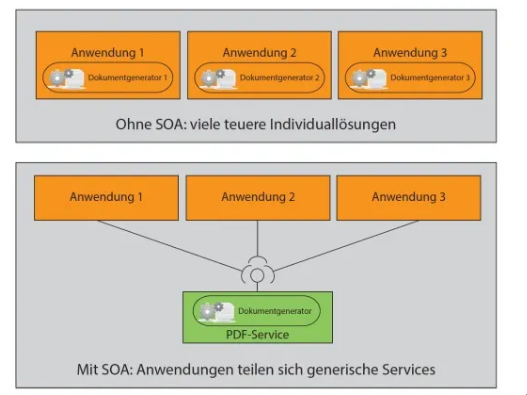
\includegraphics[width=4in,height=2in]{soa.png}
\end{center}
Die Abbildung stellt den Ansatz dar, den das SOA-Architekturmuster verfolgt. Anwendungen werden dabei in wiedervendbare Dienste aufgeteilt (Service; to not repeate Code) und so koordiniert, dass der Zweck der übergeordneten Anwendung erfüllt wird. damit wird der für eine komplexe Anwendung neu zu entwickelnde Code minimiert und dadurch die Entwicklung beschleunigt. Dieses Prinzip wird immer wieder auf verschiedenen Ebenen innerhalb der Informationstechnologie angewendet. Auf der Ebene der IT-Infrastruktur werden nach dem SOA-Prinzip z.B Datenbanken und Webserver so koordiniert, dass diese eine Platform für eine Unternehmenssoftware bilden. Daher werden standardisierte Datenbankserver für mehrere Anwendungen gleichzeitig genutzt und nicht für jede neue Anwendung ein neuer Datenbankserver in Betrieb genommen. \newline


\vspace{3mm}
Um die Wiedervendbarkeit von webbasierten Diensten zu erhöhen, wurden Protokolle entwickelt, über die Anwendungen mit webbasierten Diensten kommunizieren können. Zwei dieser Protokolle sind SOAP und XML-RPC. Beide Protokolle basieren auf XML und dienen dazu, Daten zwischen verschiedenen Systemen auszutauschen und Prozeduren auf entfernten Systeme aufzurufen.

\section{PaaS als SOA-Nachfolger}
Durch SOA sollten die Entwicklung von Unternehmensanwendungen beschleunigt und Kosten verringert werden. Tatsächlich wurden in den meisten Fällen die Kosten höher und die Entwicklungszeit länger, da zusätzliche Arbeit in die Standardisierung des Codes gesteckt werden musste und die Wiederverwendbarkeit nur selten zum Tragen kann. \newline
PaaS soll kostengünstiger und schneller vonstattengehen. Zusätzlich soll die Platform, auf der die Anwendung ausgeführt wird, automatisch skalieren und nur so viel Ressourcen in Rechnung gestellt werden, wie tatsächlich verbraucht werden. Der Entwickler soll sich nicht mehr um Infrastrukturthemen, wie die Bereitstellung von Servern, Laufzeitumgebungen und Speicherplatz kümmern müssen. Die IT-Infrastruktur wird für den Anwendungsentwickler unsichtbar (durch Abstraktion verborgen) un er kann sich auf seine eigentliche Aufgabe, die Entwicklung seiner Anwendung, konzentrieren.
\begin{center}
	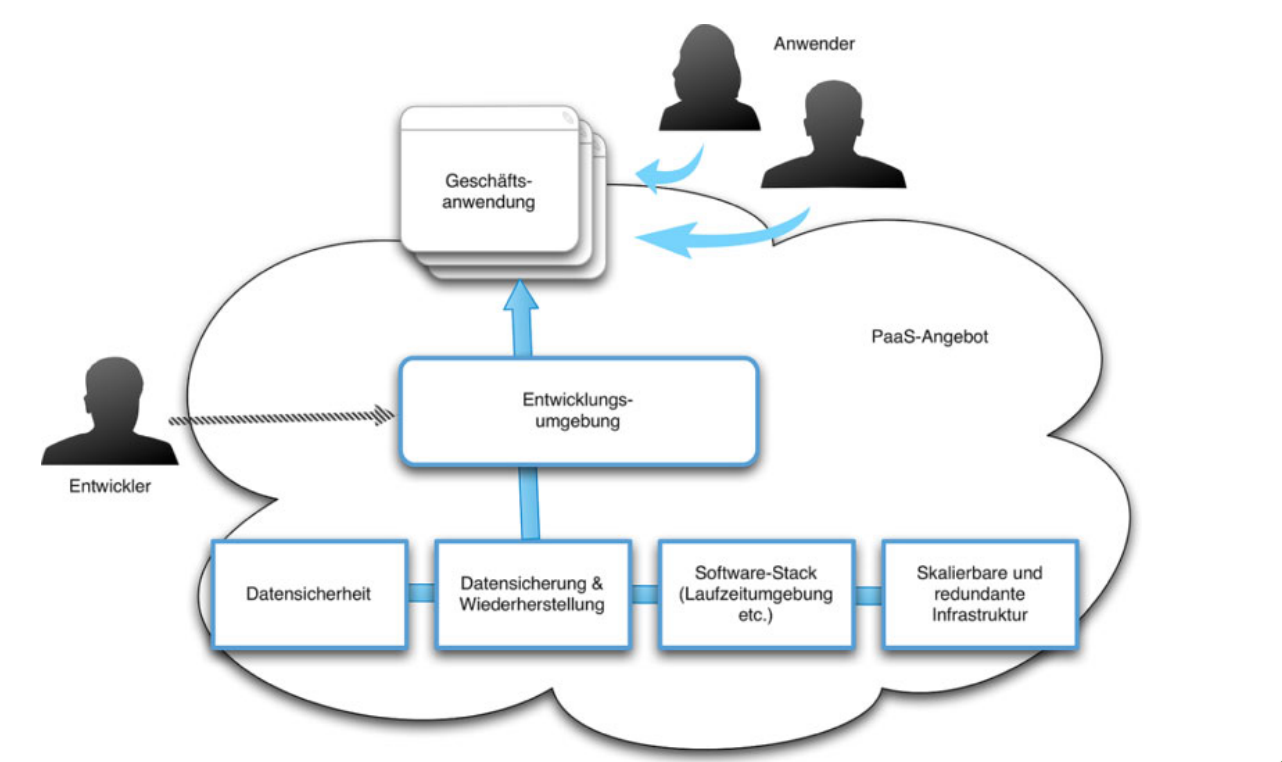
\includegraphics[width=4in,height=2in]{paas.png}
\end{center}
Fest steht das der Erfolg von SOA durch die zusätzliche komplexität, die durch die Strukturierung der einzelnen webbasierten Dienste hervorgerufen wird, stark gebremst worden ist. PaaS-Angebote verstecken diese Komplexität, die durch die Strukturierung der einzelnen webbasierten Dienste hervorgerufen wird, stark gebremst worden ist. PaaS-Angebote verstecken diese komplexität in ihren vorgefertigten APIs und bürden dem Entwickler keine zusätzlichen Aufgaben auf. Aus diesem Grund wird PaaS ein größerer Erfolg als SOA vorausgesagt. \newline


\vspace{3mm}
PaaS hat aber auch einen entscheidenden Nachteil gegenüber dem damaligen SOA-Ansatz: Anwendungen, die auf einem PaaS-Angebot ausgeführt werden, werden nicht auf eigenen Servern ausgeführt, sondern in der Cloud, deswegen eignen sich bisher nur für sich abgeschlossene Anwendungen, die nicht auf Live-Daten aus dem eigenen Rechenzentrum zugreifen müssen. Dies ist ähnlich zu SaaS-Angeboten. Im Vergleich zu SaaS sind PaaS-Angebote aber ein wenig flexibler, da die eigentliche Anwendung in Regel erst entwickelt oder angepasst werden muss und somit mehr Raum für Schnittstellen zum Datenaustausch mit dem eigenen Rechenzentrum vorhanden sind.

\section{PaaS-Typen}
PaaS-Angebote unterscheiden sich in ihrem Anwendungszweck, den Laufzeitumgebungen für verschiedene Programmiersprachen, verschiedene Datenspeichermethoden (datenbanken, etc.) und den verschiedenen Entwicklungswerkzeugen. PaaS kann man in die folgenden drei Kategorien einordnen:
\begin{itemize}
	\item aPaaS - Application PaaS
	\item iPaas - Integration and Governance PaaS
	\item Add-on-Entwicklungsumgebungen
\end{itemize}
Standardtyp bei PaaS ist aPaas. Es handelt sich dabei um die Bereitstellung einer Platform zur Entwicklung und Ausführung einer Anwendung. Bekannte Beispiele dieses PaaS-Typs sind Microsoft Azure, force.com oder Heroku. iPaaS hingegen stellt klassische Middleware-Dienste(Meta-Verzeichnise, die Daten zwischen mehreren Verzeichnisdiensten z.B Datenbank und Active Directory miteinander synchronisieren) bereit und vermittelt Daten zwischen verschiedenen Plattformen und On-Premise sowie Off-Premise-Anwendungen. Das bekannteste iPaas-Angebot ist Mule iON. Add-on-Entwicklungsumgebungen sind Erweiterungen von Saas-Angeboten um eigene Funktionen zu erweitern. Dies ist vergleichbar mit der Möglichkeit, Makros in Microsoft-Office-Anwendungen zu erstellen.
\section{Architektur von Anwendungen auf PaaS}
Eine moderne Anwendung in einem PaaS-Angebote besteht aus drei Teilen:
\begin{itemize}
	\item grafische Benutzeroberfläche: Darstellung der Daten und bietet dem Nutzer Möglichkeiten
	\item Anwendung (Web-Service): eigentliche Anwendung die aus Prozeduren und Funktionen zur Datenbearbeitung diesnt. Wird in der Regel als Web-Service implementiert. Diese WEb-Services habe definierte Ein- und Ausgabe-Parameter und werden die gewünschten Berechnungen auf die Daten an.
	\item permanenter Datenspeicher: Zur permanenten Speicherung der Daten einer Anwendung werden in Paas Angebote verschiedene Technologien Angeboten
		\begin{itemize}
			\item SQL Datenbanken: Häufig in On-Premise-Unternehmensanwendungen  verwendet. SQL Datenbanken können zwar geclustert werden aber mit jedem zusätzlichem Cluster-Knoten dauern Transaktionen Länger. Darum werden neben SQL Datenbanken auch No-SQL Datenbanken angeboten.
			\item No-SQL Datenbanken: Diese Datenbanken folgen nicht dem ACID-Prinzip (Atomarität, Konistenz, Isolation und Dauerhaftigkeit; beschreibt gewünschte Eigenschaften von Verbreitungsschritten in Datenbanksystemen), sondern arbeiten nach dem BASE-Prinzip (Datenbankänderungen werden nicht sofort, sondern nachgelagert repliziert, was in einer nachgelagerten aber trotzdem garantierten Konistenz mündet), das auf eine sofortige Konsistenz verzichtet, aber immer eine schlussendliche Konsistenz herstellt. daher sind nach einer möglichst kurzen Zeitspanne alle Knoten des No-SQL-Clusters wieder konsistent.
			\item SQL und No-SQL eignen sich nur bedingt zu Speicherung von großen Datenblöcken (sogennanten BLOBS). Aus diesem Grund bieten viele PaaS-Anbieter so genannte BLOB-Speicherdienst an.
			\item BLOB-Speicher: Lädt man eine Datei in einem BLOB-Speicherdienst hoch (dies geschiet immer über einen Funktionsaufruf aus der entsprechenden API), so erhält man als Rückgabenwert einen BLOB-Schlüssel, über den die Datei später wieder heruntergeladen werden kann. Häufig wird dieser BLOB-Schlüssel dann in der zur Anwendung gehörenden SQL-oder No-SQL-Datenbank gespeichert. Einder der bekanntessten BLOB-Speicherdienste ist Amazon S3 (Simple Storage Service)
		\end{itemize}
\end{itemize}
\begin{center}
	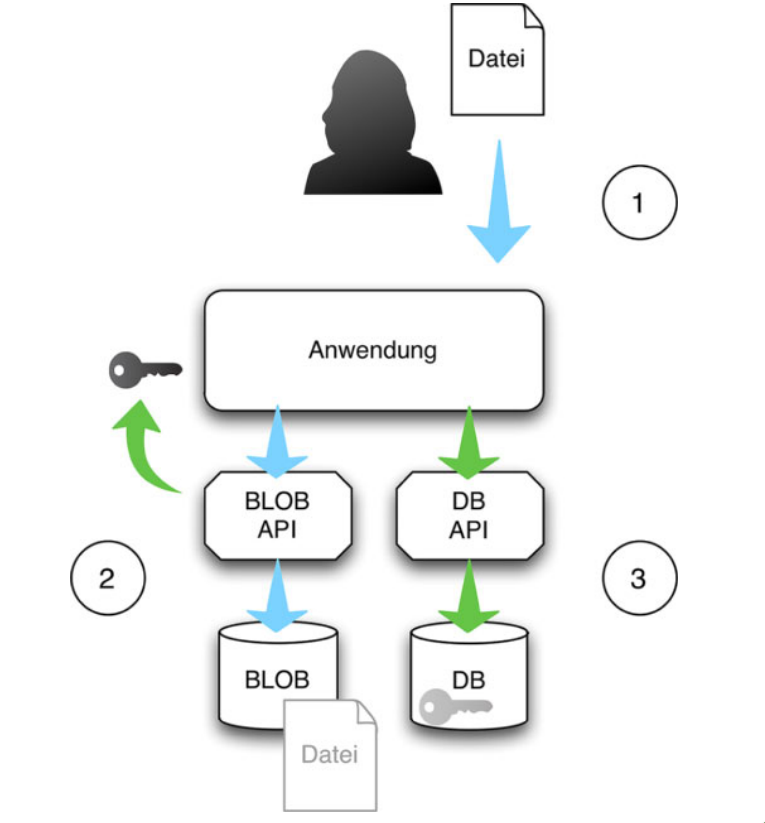
\includegraphics[width=5in,height=3in]{blob.png}
\end{center}
Zur Beschleunigung von Datenzugriffen wird von vielen PaaS-Anbietern zusätzlich ein MemCached-Dienst angeboten. Dieser Dienst wird durch Cache-Server bereitgestellt, die Datenbankinhalte und BLOBS in RAM vorhalten. Ist der Hauptspeicher des Servers voll, werden die im Cache enthaltenen Daten nach und nach gelöscht. Dabei werden zuerst die Daten gelöscht die am wenigsten zugegriffen worden sind. Hierduch werden Festplattenzugriffe vermieden und die gesamt Anwendung stark beschleunigt.
\section{Verfügbarkeit von Anwendungen auf PaaS}
Für die Verfügbarkeit einer Awendung müssen die drei Teile der Anwendung (grafische Benutzeroberfläche, Anwendung und der permanente Datenspeicher) berücksichtigt werden. Die Verfügbarkeit wird anhand der Zeit, die das System nicht verfügbar ist, und der Gesamtzeit berechnet:
$$ Verguegbarkeit=(Gesamtzeit-Gesamtausfallzeit)/Gesamtzeit $$

Der Maximalwert der Verfügbarkeit ist 1 (entspricht 100\%) und das Minimum ist 0-- wen die Gesamtausfallzeit der Gesamtzeit entspricht. Stellt man die obige Gleichung um, so erhält man mit $ Gesamtzeit*Veruegbarkeit $ eine kurze Formel, mit deren Hilfe man die Zeit ausrechnen kann, die das System mindestens verfügbar sein soll. Dies ist aus Kundensicht interessant.


\vspace{3mm}
Mit einer weiteren einfachen Umstellung der Gleichung erhält man schließlich die (für den Anbieter wichtige) vom Kunden tolerierte Gesamtlaufzeit:
$$ Gesamtausfallzeit = Gesamtzeit - Gesamtzeit * Verfuegbarkeit $$
Die Gesamtausfallzeit sellt für den Anbieter eines Dienstes die Zeit dar, die er zur Verfügung hat, um bei einem Ausfall den Diesnt wieder zur Verfügung zu stellen. Als Beispiel berechnen wir einmal die Gesamtausfallzeit bei einer Verfügbarkeit von 99\% über ein Jahr (365 Tage).

$$ Gesamtausfallzeit = 365t - 365t * 0.99 = 365t - 361,35 = 3,65t $$ \newline


\vspace{3mm}
Die Darstellung einer webbasierten Anwendung wird von Webbservern bereitgestellt, die die dazustellenden Daten von Web-Services abrufen und zusammen mit HTML-Dateien und verschiedenen Medien an den Webbrowser des Nutzers ausliefern. Die Verfügbarkeit von Serversystemen kann generell durch Redundanz erhöht werden:
\begin{itemize}
	\item Lastverteilung
		\begin{itemize}
			\item Eine Lastverteilung wird durch das Vorschalten eines sogennanten Lastverteilers erreicht. Der Lastverteiler nimmt die Anfragen der Nutzer entgegen und verteilt diese nach bestimmten Algorithmen auf die angeschlossenen Serversysteme.
		\end{itemize}


	\item Clusterbildung
		\begin{itemize}
			\item Bei einem Ausfall eines der geclusterten Serversysteme können die verbleibenden Serversysteme die Berechnung des ausgefallenen Systems übernehmen, da die Zustände aller offenen Berechnungen ständig zwischen den Systemen synchronisiert werden. Clustering verbacuht wohl mehr ressourcen und ist komplexer.
		\end{itemize}
\end{itemize}

\section{Kompatibilität}
Jeder PaaS-Anbieter sollte die Kompatibilität zu anderen Anbieter berücksichtigen. Denn wenn der Paas-Anbieter die Türen dicht macht oder der Kunde einen besseren Dienst findet soll es möglichst einfach sein, die Anwendung samt Daten zu einem anderen PaaS-Anbieter oder in ein eigenes Rechenzentrum zu migrieren. Diese kompatibilität muss auf mehreren Ebenen geprüft werden wie die Programmierpsrache der Laufzeitumgebung, Anpassungen an der API können notwendig sein oder der Anbieter bietet eine gleiche API an. Weiterhin muss der vom neuen PaaS-Anbieter bereitgestellte permanente Speicher zu dem alten Speicher kompatibel sein. Hierbei sind die APIs für den Zugriff auf den Speicherdienst zu beachten auf ihre Kompatibilität. Anderfalls müssen selbst Anpassungen stattfinden. Viele PaaS-Nutzer verwenden aufgrund hoher Kompatibilitätsanforderungen verschiedene PaaS-Anbieter für die Laufzeitumgebung und den permanenten Speicher. Dadurch wird die Abhängikeit zu den PaaS-Anbietern etwas verringert.
\subsection{Aufgaben}
1.1 - Richtig \newline
1.2 - Beschaffen von Hardware, Bereitstellung von Servern und laufzeitumgebungen, Datenbanken, Datensicherung und Wiederherstellung. bzw. Infrakstrukture und Software-stack \newline
1.3 - aPaas - Application PaaS \newline
1.4 - Die zwei arten von Benutzeroberflächen sind:  Webbasierte Oberfkächen und mobile Anwendungen für Smartphones\newline
1.5 - die Gesamtausfallzeit läßt sich mit der Formal $ Gesamtausfallzeit = Gesamtzeit - Gesamtzeit * Verfuegbarkgeit $ \newline
1.6 - Falsch \newline

















\end{document}
